\begin{center}
	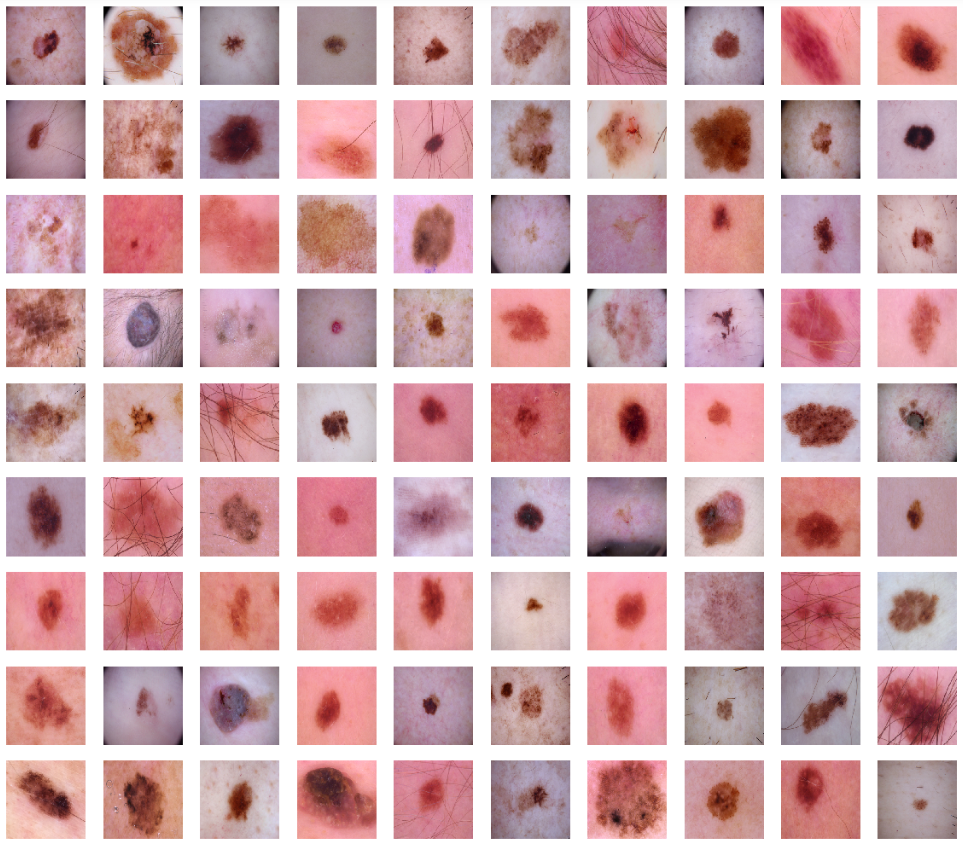
\includegraphics[width=10cm]{Images/bseg.png}
\end{center}

The figure above reflects the sample from training dataset before performing image segmentation.
The image segmentation was performed on the all the images using binary thresholding in OpenCV framework.

\section{Thresholding Segmentation Algorithm}

Thresholding is one of the commonly adopted method in image segmentation which helps in descrimination most 
significant pixels in the images \citep*{al2010image}. The thresold value is selected and the gray scale images  
are converted into the binary representation of the image and value of image which are greater than the thresold
value will be selected with keeping all the attributes of the images such as position and shape \citep*{al2010image}. 
Thus, reducing the complexity of the image data and making it easier for classification related tasks. Futhermore, the 
segmented images will be consumed in the model training. The thresholding segmentation was performed using OpenCV library using 
\url{cv.threshold(image, 0.5, 1, cv.THRESH_BINARY)} where threshold value of 0.5 and maximum value of the pixel can be 1
as it was normalised.

\begin{center}
	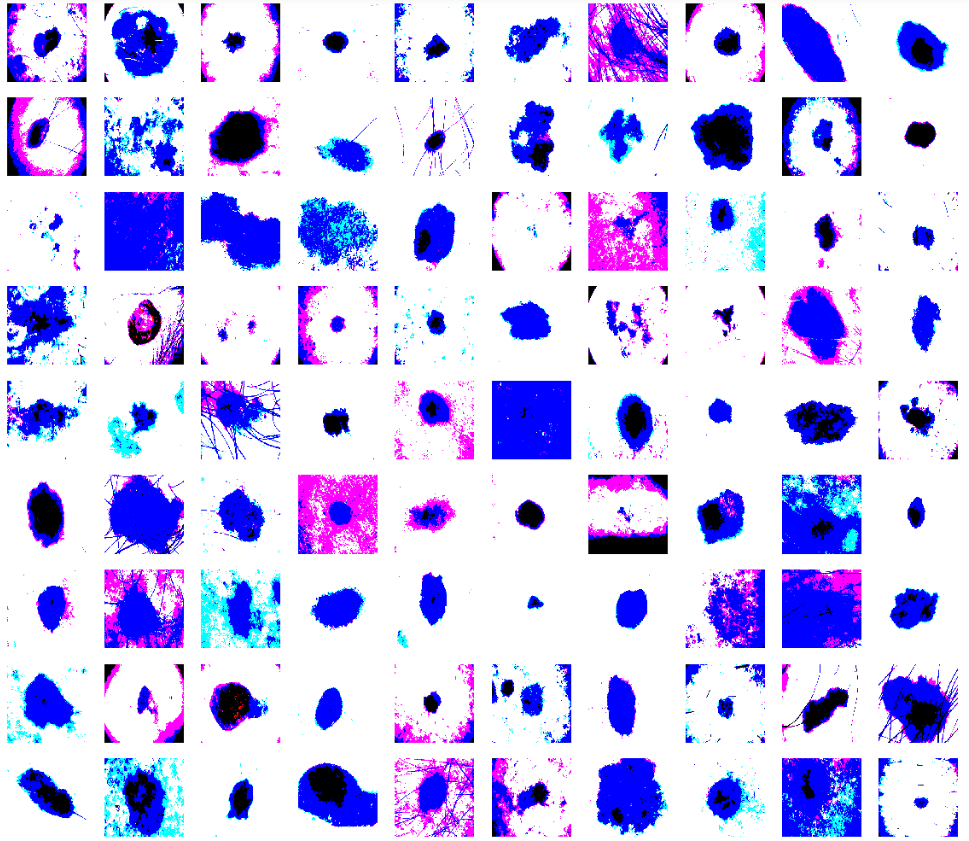
\includegraphics[width=10cm]{Images/aseg.png}
\end{center}

The figure above shows the result of applying the threshold image segmentation on pigmented skin lesions. 
